\documentclass{scrartcl}

\usepackage{tikz}
\usetikzlibrary{matrix.skeleton}

\usepackage[justification=centering,labelfont={sf,bf,up},labelsep=period,font=small]{caption}
\captionsetup[figure]{position=bottom,singlelinecheck=false}
\usepackage[font=small,justification=centering]{subcaption}
\usepackage{float}
\floatstyle{komabelow}
\restylefloat{figure}

\usepackage{xspace}

\usepackage{hyperref}
\hypersetup{ colorlinks=true
           , linkcolor=blue!75
           , citecolor=black
           , urlcolor=blue!75
           }

\usepackage[noabbrev, capitalize]{cleveref}

\tikzset{highlight/.style={draw=#1!75, fill=#1!25, rounded corners=1pt}}
\newcommand\code\texttt
\newcommand{\TikZ}{Ti\textit{k}Z\xspace}

\title{\texttt{matrix.skeleton}'s Manual}
\author{Nicolas Dudebout}
\date{}

\begin{document}

\maketitle

\section{Introduction}

The \TikZ \code{matrix} library places nodes on a grid.
However, this grid is discarded after the nodes have been placed.
As a result, certain constructions involving multiple nodes become cumbersome.
The following two examples highlight some of the difficulties.

\subsection{Alignment Issues with \code{fit}}

The \code{fit} library is used to highlight a subset of nodes in a matrix.
If all the nodes in the matrix have the same dimension, as in~\cref{fig:highlighting_identical_dimensions}, \code{fit} produces the desired output.

\begin{figure}[h]
\centering

\begin{subfigure}{0.45\textwidth}
\centering
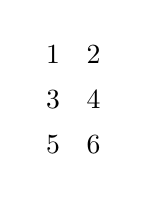
\begin{tikzpicture}
\matrix (m) [matrix of math nodes, column sep = 3pt, row sep = 3pt] {
1 & 2 \\
3 & 4 \\
5 & 6 \\
};
\end{tikzpicture}
\caption{Input matrix}
\end{subfigure}
%
\begin{subfigure}{0.45\textwidth}
\centering
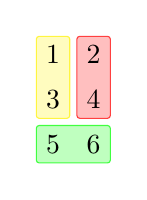
\begin{tikzpicture}
\matrix (m) [matrix of math nodes, column sep = 3pt, row sep = 3pt] {
1 & 2 \\
3 & 4 \\
5 & 6 \\
};

\fitandstyle[background]{(m-1-1) (m-2-1)}{highlight = yellow}
\fitandstyle[background]{(m-1-2) (m-2-2)}{highlight = red}
\fitandstyle[background]{(m-3-1) (m-3-2)}{highlight = green}
\end{tikzpicture}
\caption{Desired output and result with \code{fit}}
\end{subfigure}

\caption{Highlighting in a matrix with nodes of identical dimensions}
\label{fig:highlighting_identical_dimensions}
\end{figure}

However, if the nodes have different heights and widths, as illustrated in~\cref{fig:highlighting_different_dimensions}, some alignment issues arise.

\begin{figure}[h]
\centering
\begin{subfigure}{0.3\textwidth}
\centering

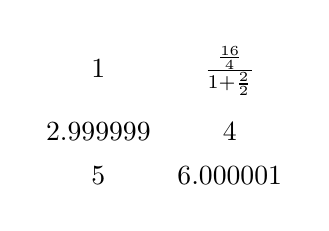
\begin{tikzpicture}
\matrix (m) [matrix of math nodes, column sep = 3pt, row sep = 3pt] {
1        & \frac{\frac{16}{4}}{1 + \frac{2}{2}} \\
2.999999 & 4                                    \\
5        & 6.000001                             \\
};
\end{tikzpicture}
\caption{Input matrix}
\end{subfigure}
%
\begin{subfigure}{0.3\textwidth}
\centering

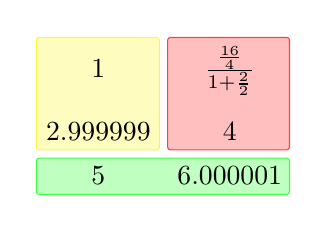
\begin{tikzpicture}
\matrix (m) [matrix of math nodes, column sep = 3pt, row sep = 3pt, label skeleton] {
1        & \frac{\frac{16}{4}}{1 + \frac{2}{2}} \\
2.999999 & 4                                    \\
5        & 6.000001                             \\
};

\fitandstyle[background]{(m-cell-1-1) (m-cell-2-1)}{highlight = yellow}
\fitandstyle[background]{(m-cell-1-2) (m-cell-2-2)}{highlight = red}
\fitandstyle[background]{(m-cell-3-1) (m-cell-3-2)}{highlight = green}
\end{tikzpicture}
\caption{Desired output}
\end{subfigure}
%
\begin{subfigure}{0.3\textwidth}
\centering

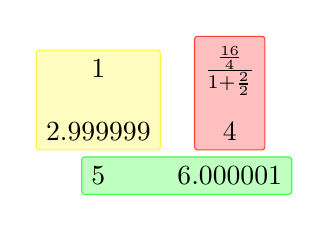
\begin{tikzpicture}
\matrix (m) [matrix of math nodes, column sep = 3pt, row sep = 3pt] {
1        & \frac{\frac{16}{4}}{1 + \frac{2}{2}} \\
2.999999 & 4                                    \\
5        & 6.000001                             \\
};

\fitandstyle[background]{(m-1-1) (m-2-1)}{highlight = yellow}
\fitandstyle[background]{(m-1-2) (m-2-2)}{highlight = red}
\fitandstyle[background]{(m-3-1) (m-3-2)}{highlight = green}
\end{tikzpicture}
\caption{Result with \code{fit}}
\end{subfigure}

\caption{Highlighting in a matrix with nodes of different dimensions}
\label{fig:highlighting_different_dimensions}
\end{figure}

These problems can be addressed using \code{minimum width} and \code{minimum height}.
However, adjusting manually these parameters in every matrix is a waste of time.

The \code{matrix.skeleton} library provides a clean solution through the use of nodes called~\code{cells}.
These \code{cells} and other skeleton nodes are described in~\cref{sec:skeleton}.

\subsection{Working with Rows and Columns}

The readability of a matrix can sometimes be improved by adding a background on every other row.
This simple task is not easily achievable with \code{matrix} alone.
The style \code{every odd column} only affects the nodes of the said columns.
There is no real column object to work with.

The \code{matrix.skeleton} library provides \TikZ styles to achieve this goal easily.
These styles are described in~\cref{sec:styling}

\section{Skeleton}
\label{sec:skeleton}

\subsection{Nodes}

\code{matrix.skeleton} works by positioning a set of nodes to recreate the \code{matrix} grid.
The eight types of such nodes are illustrated in~\cref{fig:skeleton_nodes}.

\begin{figure}[h]
\centering
\begin{subfigure}{0.3\textwidth}
\centering
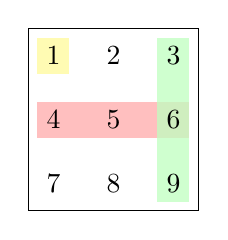
\begin{tikzpicture}
\matrix (m) [draw, matrix of nodes, column sep=10pt, row sep=10pt, label skeleton] {
1 & 2 & 3 \\
4 & 5 & 6 \\
7 & 8 & 9 \\
};

\fitandstyle[background]{(m-cell-1-1)}{fill=yellow!30}
\fitandstyle[background]{(m-row-2)}{fill=red!25}
\fitandstyle[background]{(m-column-3)}{fill=green!25, opacity=.75}
\end{tikzpicture}
\caption{\textcolor{yellow!80!orange}{Cell}, \textcolor{red!50}{row}, and \textcolor{green!60}{column}}
\end{subfigure}
%
\begin{subfigure}{0.3\textwidth}
\centering
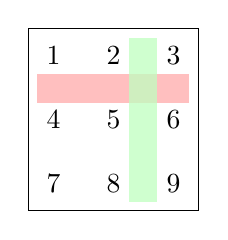
\begin{tikzpicture}
\matrix (m) [draw, matrix of nodes, column sep=10pt, row sep=10pt, label skeleton] {
1 & 2 & 3 \\
4 & 5 & 6 \\
7 & 8 & 9 \\
};

\fitandstyle[background]{(m-inter-row-1)}{fill=red!25}
\fitandstyle[background]{(m-inter-column-2)}{fill=green!25, opacity=.75}
\end{tikzpicture}
\caption{\textcolor{red!50}{Inter-row} and \textcolor{green!60}{inter-column}}
\end{subfigure}
%
\begin{subfigure}{0.3\textwidth}
\centering
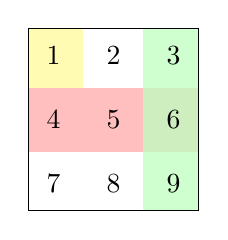
\begin{tikzpicture}
\matrix (m) [draw, matrix of nodes, column sep=10pt, row sep=10pt, label skeleton] {
1 & 2 & 3 \\
4 & 5 & 6 \\
7 & 8 & 9 \\
};
\fitandstyle[background]{(m-tiling-cell-1-1)}{fill=yellow!30}
\fitandstyle[background]{(m-tiling-row-2)}{fill=red!25}
\fitandstyle[background]{(m-tiling-column-3)}{fill=green!25, opacity=.75}
\end{tikzpicture}
\caption{\textcolor{yellow!80!orange}{Tiling cell}, \textcolor{red!50}{tiling row}, and \textcolor{green!60}{tiling column}}
\end{subfigure}
\caption{Skeleton nodes}
\label{fig:skeleton_nodes}
\end{figure}

\subsection{Using \code{matrix.skeleton}}

The recommended way of using \code{matrix.skeleton} is through \TikZ.
First, load the library with:
\begin{verbatim}
  \usetikzlibrary{matrix.skeleton}
\end{verbatim}
Then add an option to your matrix:
\begin{verbatim}
  \matrix (m) [label skeleton] {...};
\end{verbatim}
This creates a set of nodes that can be used for styling.
For example, the nodes illustrated in~\cref{fig:skeleton_nodes} are named: \code{m-cell-1-1}, \code{m-row-2}, \code{m-column-3}, \code{m-inter-row-1}, \code{m-inter-column-2}, \code{m-tiling-cell-1}, \code{m-tiling-row-2}, and \code{m-tiling-column-3}.

\section{Styling}
\label{sec:styling}

The skeleton nodes are PGF nodes not meant to be styled.
Styles should be applied to nodes whose shapes depend on the skeleton ones.

\subsection{Macros}

Styling in \code{matrix.skeleton} is done with the~\code{fit} library.
The following macro creates a \code{fit} node with the specified style:
\begin{verbatim}
  \fitandstyle{(m-cell-1-1) (m-cell-2-2)}{draw=red};
\end{verbatim}

It takes an optional argument to place the node in a \code{pgfonlayer} environment:
\begin{verbatim}
  \fitandstyle[background]{(m-cell-1-1) (m-cell-2-2)}{fill=red};
\end{verbatim}

\subsection{\TikZ \code{matrix} Options}

Common styling options are also provided as \TikZ options.
These options call~\code{label skeleton} before styling the appropriate nodes.
They take the following form:
\begin{verbatim}
  \matrix (m) [style odd rows = {draw=red}] {...};
\end{verbatim}

\begin{verbatim}
  \matrix (m) [style odd tiling rows = {draw=red}] {...};
\end{verbatim}

\begin{verbatim}
  \matrix (m) [style grid = {draw}] {...};
\end{verbatim}

\begin{verbatim}
  \matrix (m) [style tiling grid = {draw}] {...};
\end{verbatim}

All of these options have an \code{on layer} variant taking the following form:
\begin{verbatim}
  \matrix (m) [style odd rows on layer = {background}{fill=red}] {...};
\end{verbatim}

\section{Examples}

The following examples illustrate the styling capabilities offered by \code{matrix.skeleton}.

\subsection{Grid}

\begin{figure}[h]
\centering
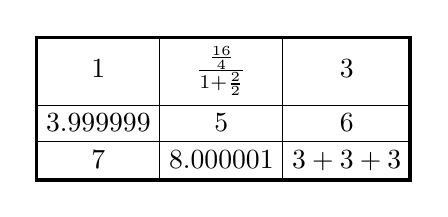
\begin{tikzpicture}
\matrix (m) [matrix of math nodes, style contour = {draw, very thick}, style grid = {draw, thin}] {
1        & \frac{\frac{16}{4}}{1 + \frac{2}{2}} & 3         \\
3.999999 & 5                                    & 6         \\
7        & 8.000001                             & 3 + 3 + 3 \\
};
\end{tikzpicture}
\end{figure}

\begin{verbatim}
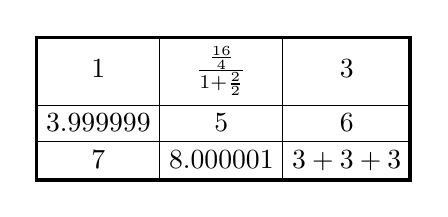
\begin{tikzpicture}
\matrix (m) [matrix of math nodes, style contour = {draw, very thick},
             style grid = {draw, thin}] {
1        & \frac{\frac{16}{4}}{1 + \frac{2}{2}} & 3         \\
3.999999 & 5                                    & 6         \\
7        & 8.000001                             & 3 + 3 + 3 \\
};
\end{tikzpicture}
\end{verbatim}

\subsection{Rows}

\begin{figure}[h]
\centering
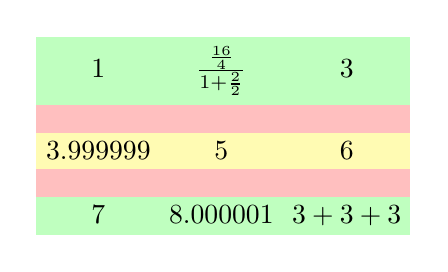
\begin{tikzpicture}
\matrix (m) [matrix of math nodes, row sep = 10pt, style odd rows on layer={background}{fill=green!25}, style even rows on layer={background}{fill=yellow!30}] {
1        & \frac{\frac{16}{4}}{1 + \frac{2}{2}} & 3         \\
3.999999 & 5                                    & 6         \\
7        & 8.000001                             & 3 + 3 + 3 \\
};

\fitandstyle{(m-inter-row-1)}{fill=red!25}
\fitandstyle{(m-inter-row-2)}{fill=red!25}
\end{tikzpicture}
\end{figure}

\begin{verbatim}
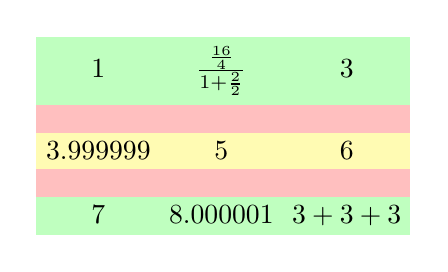
\begin{tikzpicture}
\matrix (m) [matrix of math nodes, row sep = 10pt,
             style odd rows on layer={background}{fill=green!25},
             style even rows on layer={background}{fill=yellow!30}] {
1        & \frac{\frac{16}{4}}{1 + \frac{2}{2}} & 3         \\
3.999999 & 5                                    & 6         \\
7        & 8.000001                             & 3 + 3 + 3 \\
};

\fitandstyle{(m-inter-row-1)}{fill=red!25}
\fitandstyle{(m-inter-row-2)}{fill=red!25}
\end{tikzpicture}
\end{verbatim}

\subsection{Checker Board}

This example is inspired by the following \href{http://tex.stackexchange.com}{\TeX{} - \LaTeX{} Stack Exchange} question: \href{http://tex.stackexchange.com/questions/14061/how-can-i-set-the-background-color-of-the-rows-and-columns-of-a-matrix-node-in-t}{How can I set the background color of the rows and columns of a matrix node in Tikz?}

\begin{figure}[h]
\centering
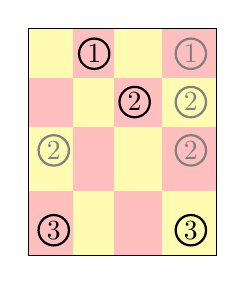
\begin{tikzpicture}
\matrix (m) [draw, matrix of nodes, row sep=2mm, column sep=1mm, nodes={draw, thick, circle, inner sep=1pt}, label skeleton] {
  & 1 & &[2mm]|[gray]|1\\
  & & 2 &|[gray]|2\\
  |[gray]|2 & & &|[gray]|2\\[4mm]
  3 & & & 3\\
};
\foreach \row in {1, ..., 4} {
  \foreach \col in {1, ..., 4} {
    \pgfmathparse{Mod(\row + \col, 2) ? "red!25" : "yellow!30"}
    \colorlet{squarebg}{\pgfmathresult}
    \fitandstyle[background]{(m-tiling-cell-\row-\col)}{fill = squarebg}
  }
}
\end{tikzpicture}
\end{figure}

\newpage

\begin{verbatim}
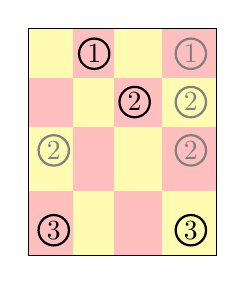
\begin{tikzpicture}
\matrix (m) [draw, matrix of nodes, row sep=2mm, column sep=1mm,
             nodes={draw, thick, circle, inner sep=1pt}, label skeleton] {
  & 1 & &[2mm]|[gray]|1\\
  & & 2 &|[gray]|2\\
  |[gray]|2 & & &|[gray]|2\\[4mm]
  3 & & & 3\\
};
\foreach \row in {1, ..., 4} {
  \foreach \col in {1, ..., 4} {
    \pgfmathparse{Mod(\row + \col, 2) ? "red!25" : "yellow!30"}
    \colorlet{squarebg}{\pgfmathresult}
    \fitandstyle[background]{(m-tiling-cell-\row-\col)}{fill = squarebg}
  }
}
\end{tikzpicture}
\end{verbatim}

\section{Internals}

\code{matrix.skeleton} was heavily inspired by \href{http://tex.stackexchange.com/users/86/andrew-stacey}{Andrew Stacey}'s \code{matrixcells} \LaTeX{} package.
It has three distinctive features.
First, it works with any \code{anchor}.
Second, it provides finer control with respect to \code{row sep}, \code{column sep}, and \code{inner sep}.
Third, the skeleton node positioning relies only on \TeX and PGF, not on \LaTeX{} or \TikZ.

\code{matrixcells} properly aligns its \code{cells} when the node \code{anchor} is \code{center}.
However, when the alignment is different it runs into problems, as exposed in the following \href{http://tex.stackexchange.com}{\TeX{} - \LaTeX{} Stack Exchange} question: \href{http://tex.stackexchange.com/questions/128045/matrixcells-problem-with-the-y-axis-only}{Matrixcells problem with the y-axis only}.
This shortcoming is the result of some loss of information in \code{pgfmodulematrix.code.tex}.
A dimension used during the placement of nodes is overwritten.
Therefore, this information is not available to build the grid.
In \code{matrixcells}, this lost dimension is reconstructed as the average of two other dimensions.
This method only gives the right dimension when the nodes are centered.
To always get proper alignment, the~\code{pgfmodulematrix.code.tex} macro erasing the dimension was rewritten.
Following \href{http://tex.stackexchange.com/users/3235/percusse}{\code{@percusse}}'s recommendation this change is transparent to the user and does not require updating PGF/\TikZ.

\code{matrixcells} only provides \code{cells} corresponding the \code{tiling-cells} in \code{matrix.skeleton}.
This tiling behavior is sometimes desired.
However, it can result in unexpected behaviors when: using a non-center \code{anchor}, using \code{row sep} or \code{column sep}, or when working on boundary nodes.

\end{document}